\title{Study Guide for Midterm 1}
\author{Dr. Jordan Hanson - Whittier College Dept. of Physics and Astronomy}
\date{\today}
\documentclass[10pt]{article}
\usepackage[margin=1.5cm]{geometry}
\usepackage{outlines}
\usepackage{graphicx}
\usepackage{amsmath}

\begin{document}
\maketitle

\section{Memory Bank}

\begin{itemize}
\item $T^2 = R^3$ ... Kepler's 3rd Law, if $T$ is the orbital period in years and $R$ is the orbital radius in AU.
\item $R_{AU} = D_E/\left(2\pi\Delta t (T_V^{-1} - T_E^{-1})\right)$
\item $W = F d$ ... Work (in Joules) is equal to force (in Newtons) times distance (in meters).
\item $f = \mu m g$ ... The force of friction if $f$ is in Newtons, $m$ is the mass in kilograms, and $g = 9.18$ m/s$^2$.  The number $\mu$ is called the coefficient of friction.
\item $W = \mu m g d$ ... Combining the above two formulas, we find the work in pulling a load against friction for some distance.
\item $W = mgh$ ... The work required to ascend a height $h$ carrying a mass $m$.
\item 1 kilocalorie, or 1 kcal, is equal to 4184 Joules.
\item The following conversions are useful: 1 gram of fat has 9 kcal of energy.  1 gram of protein has 4 kcal of energy.  1 gram of carbohydrate has 4 kcal of energy.
\item A distance \textit{vector} can be expressed as an amount of distance in a given direction.  We use the notation $\vec{x} = (a,b)$ to represent the amount of distance East ($a$), and the amount of distance North ($b$).
\item Vectors add like lists of numbers: $(a,b) + (x,y) = (a+x,b+y)$.
\item To calculate the \textit{length} of a vector $|\vec{x}|$, we use the Pythagorean theorem: $|\vec{x}| = \sqrt{a^2+b^2}$
\item To calculate the \textit{angle} $\theta$ a vector makes with the x-axis, we use trigonometry: $\theta = \tan^{-1}(b/a)$.
\end{itemize}

\section{The Planets}

\begin{enumerate}
\item Kepler's Third Law states that if the orbital period of a planet is given in \textit{years}, and the orbital radius is given in \textit{AU}, then 
\begin{equation}
T^2 = r^3
\end{equation}
For example, we can solve for the orbital radius like $r = T^{2/3}$.  If the period of Venus is $T=0.615$ years, then $r = (0.615)^{2/3} = 0.723$ AU.  Given the following orbital periods, solve for the orbital radii of the planets:
\begin{itemize}
\item Jupiter: 11.862 years
\item Saturn: 29.457 years
\item Pluto: 248 years
\end{itemize}
Solve for the following orbital periods:
\begin{itemize}
\item Mars: 1.524 AU
\item Uranus: 19.22 AU
\item Neptune: 30.11 AU
\end{itemize}
\end{enumerate}

\section{Work, Force, and Friction}

\begin{enumerate}
\item Recall that the unit of work is a Joule, and it is equal to a force in Newtons times a distance in meters.  Calculate the following quantities, given the initial parameters.
\begin{itemize}
\item Given that a sled is pushed with a net force of 50 N for a distance of 1000 m, how many Joules of energy does this require?
\item Suppose someone pushes the sled 2000 meters, and expends 100,000 Joules.  How far did they travel?
\item Suppose someone expends 200,000 Joules, and travels 1500 meters pushing a sled.  With how much force did they push?
\end{itemize} \vspace{3cm}
\item \textbf{Forces add together.}  Suppose two dogs, who can each pull with 75 N, are hooked to a sled.  They pull together, adding their forces.  They each expend 10,000 Joules of energy.  How far did they pull the sled? \vspace{3cm}
\item Recall that the force of friction is a numerical coefficient $\mu$ times the mass of the thing moving against it $m$ in kilograms times $g = 9.81$ m/s$^2$.  That is, $f = \mu m g$.  Suppose a sled that has 150 kg of mass is on snow, where the coefficient of friction is about 0.1.  What would be the force of friction? \vspace{3cm}
\item Suppose we have to pull a sled with whatever force is enough to equal the frictional force.  If the sled is loaded with 500 kg, and $g=9.18$ m/s$^2$, with what force will we have to pull if we encounter a) waxed wood on wet snow? b) metal on wood? c) What if we are smart and put ice on our sled skis, and pull across ice (ice on ice)?
\begin{figure}[hb]
\centering
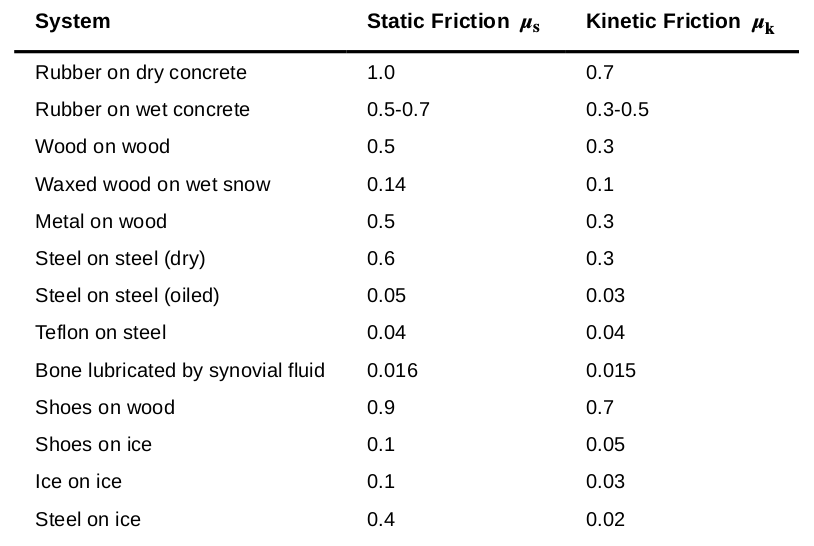
\includegraphics[width=0.45\textwidth]{friction.png}
\caption{\label{fig:friction} Frictional coefficients for different surfaces.}
\end{figure}
\item Suppose we have to pull with some force that equals friction, $f = \mu m g$, across some distance $d$.  That means we would have to do work equal to the distance times the friction force, or $W = \mu m g d$.  What work would be required if $\mu = 0.05$, $m = 1000$ kg, and $d = 20,000$ m (20 km)? \\ \vspace{3cm}
\item (Same situation as previous example).  What if instead of doing this ourselves, we get 10 dogs to do it?  How much energy per dog would be required? \\ \vspace{2cm}
\end{enumerate}

\section{Food Energy and Unit Conversion}

\begin{enumerate}
\item Suppose we need 1 MJ (1 million Joules) of energy in food.  Given that the energy density of protein is 4 kcal/gram, how many grams are required?  What is this number in kilograms? \\ \vspace{1cm}
\item Same situation, but instead of proteins, let's use the energy density of fats, which is 9 kcal/gram. \\ \vspace{1cm}
\item Suppose that half of the 1 MJ has to be carbohydrates, and half must be fats.  How many kilograms do you need of each? \\ \vspace{1cm}
\end{enumerate}

\section{Navigation}

\begin{enumerate}
\item Suppose a traveler heads North for 10 km and rests.  The next day, she heads West for 10 km.  Write her final position in vector notation. \\ \vspace{1cm}
\item (Same situation).  How far is she from where she began? \\ \vspace{1cm}
\item (Same situation).  At what angle is she heading? \\ \vspace{1cm}
\item Suppose an expedition heads North for 5 km, then turns 45 degrees to the right and goes another 5 km.  Next, they turn North again and go another 5 km.  Finally, they turn to the right by 90 degrees and go 5 km.  What is their final position? \\ \vspace{2cm}
\item (Same situation).  How far are they from the origin? \\ \vspace{1cm}
\end{enumerate}

\section{Summary}

\begin{enumerate}
\item Begin at the black diamond in the upper right corner of Fig. \ref{fig:maze}.  Chart a course for the white diamond in the lower left. Assume a friction coefficient of 0.05, and assume you are carrying 600 kg the whole time.  Assume further that the glacier at the bottom left requires climbing an elevation of 2000 m.  How much energy is required?
\begin{figure}[hb]
\centering
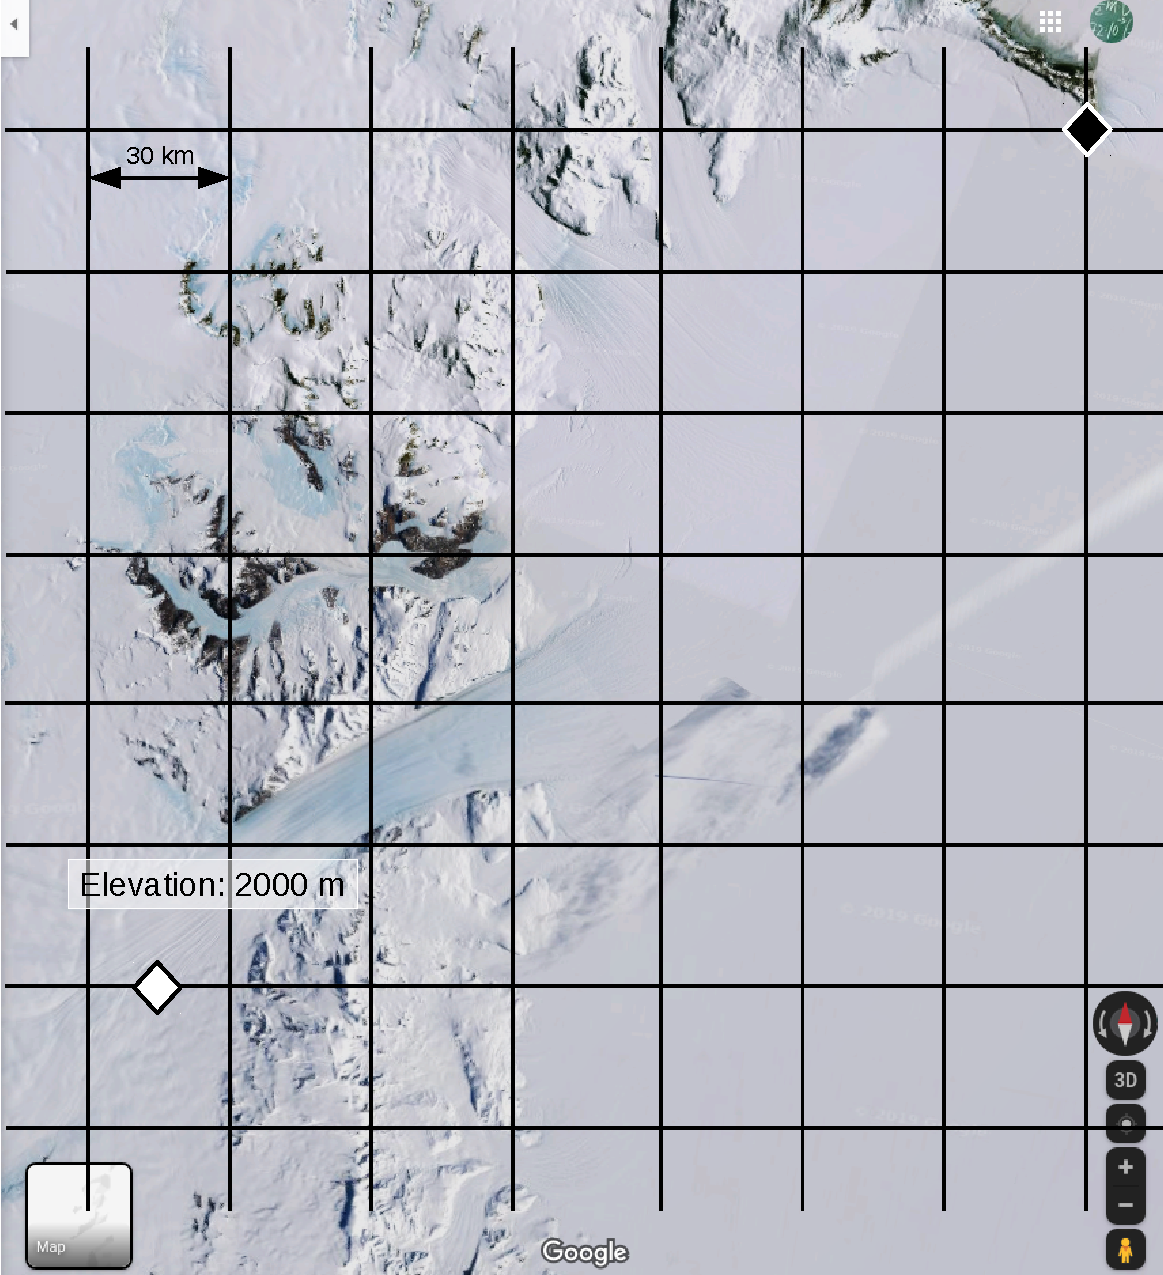
\includegraphics[width=0.5\textwidth]{glacier2.pdf}
\caption{\label{fig:maze} Map for the summary calculation.}
\end{figure}
\end{enumerate}

\end{document}
